\section{2022 Test 1 Notes}

对于每道题,请先写一遍题目中提到的定义。

\subsection{Q2}
\subsubsection{a}
软件维护的种类:corrective, adaptive, preventative, perfective。
增加一个特性是perfective。
\subsubsection{b 讨论可变性:}
可更改性是指如何在不引入缺陷或降低现有产品质量的前提下,有效且充分地更改产品系统。
4.3 中有很多地方需要修改,而 5.1 中的修改只有第 14、61、62 和 64 行(后三行都在一个方法 changePlayer() 中)。因此,仅仅修改 4.3 就需要更多的工作(\textbf{效率更低})。

由于要修改的地方较多,而每个地方都有可能出错(例如漏掉),因此要修改的地方越多,出错的可能性就越大(假设出错的可能性差不多--在本例中是一样的,因为在两种实现中要做的修改是一样的)。由于 4.3 需要改动的地方较多,在改动时出错的几率也较高,因此\textbf{有效性}较低。

提示:可变性与可理解性互相独立。本题中请不要讨论可理解性。

\subsection{Q3 类的大小/数量如何影响测试性}
比较:

小的类会比大的多(因为功能是一样的)。假设每个类都能提供相同水平的可观察性和可控制性,这意味着小的将比大的拥有更多的可观察性和可控制性,因此更容易测试。

事实上,小类可能比大类更具可观察性和可控性。类越大,需要为测试正确设置的状态就越多(Controllability),需要查看(Observability)的东西就越多,以便在测试后确认类中的对象是正确的。也就是说,需要花费更多精力来进行测试,这就不如小类的效率(Efficiency)高。

有单一责任(SRP)的类通常比没有单一责任的类小。

当一个类依赖于另一个类时(例如,通过调用另一个类中对象的方法),测试该类就需要额外的工作来设置另一个类中的对象。小类更有可能不依赖于其他类,因此所需的工作量会更少(Efficiency)。

\subsection{Q4 PCM}
\subsubsection{解释KB中的知识的特性}

这种知识优势必须存在(在知识库中),以便能够理解任何代码,但这种知识并不具体涉及所理解的代码。

String result = obj.someMethod(); 例如,对于这段代码:我们将使用 Java 语法知识来认识到 someMethod() 必须返回字符串(假设代码能编译)。知识库中的这些知识类似于 "当赋值运算符 (=) 右侧有一个方法调用,左侧有一个 java.lang.String 类型的变量时,该方法必须返回一个 String 值"。这不是专门关于代码的知识,因此不会出现在 MM 中。
MM 中的知识应该是这样的:"变量 obj 来自 A 类,A 类中的方法 someMethod() 返回一个描述对象当前状态的字符串"。

\subsubsection{解释陌生代码如何内化}
这段代码位于 ER 中。理解这段代码需要 Java 方面的知识,尤其是 = 左边和右边的含义。此外,还需要了解方法调用语法和方法调用的含义。这些知识与代码本身无关(见第(a)部分),因此必须放在知识库中。
如果您没有相关的 Java 知识,也就是说知识库中没有这些知识,那么您就需要获取这些知识。这就需要查阅有关 Java 的描述,这些描述可以在 ER 中找到。一旦掌握了这些知识,它们就会出现在知识库中。
一旦掌握了必要的 Java 知识,您就可以通过 AP 来解释代码(在 ER 中),从而确定代码的作用,并根据这些新信息更新 MM。

请注意,需要引用模型中的每一个组件。

\subsection{Q5 可读性}

\subsubsection{a 可读性如何影响可理解性}
识别元素(如循环体)或区分元素(如一个变量与另一个变量)或确定哪些元素属于同一个元素越困难,阅读就越困难。 如果阅读困难,那么理解的效果和/或效率就会降低。因此,可读性低就意味着可理解性低。

\subsubsection{b 巨量代码空白如何影响可理解性}
卫生间管道提示建议不要让多个函数的代码同时出现在屏幕上。每行之间有多个空行可能会降低可理解性,因为读者需要上下滚动屏幕来阅读和理解一个功能。如果阅读一个功能需要时间,那么从 ER 到 KB/MM 的内化过程就会延长。从而影响理解一个功能的效果和效率。


\subsection{Q6 四连棋游戏}

\subsubsection{a 棋子类是否必要}

为玩家投放到网格中的物品(从现在起将称为 "令牌")引入一个类别会增加理解该类别所需的额外工作。

不过,我们可以考虑另一种方法。必须要有一些代码来显示网格中是否有标记物。这些代码至少需要记录它属于哪个玩家,可能还需要记录它的颜色。每次有人查看这段代码时,他们都必须记住这段代码在做什么。

可维护性的定义(及其所有方面)适用于整个生命周期内的整个实现。因此,虽然在第一次查看类的代码时需要付出额外的努力,但预计在大多数情况下,这些代码都不会再被查看。从长远来看,该类的成本可能与查看备用代码并记住其含义的成本相差不大。

此外,如果需要对令牌进行任何更改(可更改性),如果有一个类,那么所需的努力将仅限于更改该类。如果只有一些代码,那么该代码存在的每个地方(例如,检查行中哪个位置未填写的代码、检查是否有中奖行的代码)都必须更改。这种工作量(效率)可能远远超过仅仅更改类的工作量。

我们需要的主要方法是一个能确定由哪位玩家出牌的方法(例如类似 getColour()的方法)。在真实游戏(上下文模式)中,没有什么能阻止玩家交换他们使用的颜色)。

\subsubsection{b “棋子”还是“令牌” - PCM}
一个类与上下文或设计模式中所代表的概念越一致,就越容易理解。鉴于问题中对游戏的描述总是提到 "令牌",这似乎比任何其他选择(包括 "棋子")都更好。

\textbf{The more a class is consistent with the concept it represents from the context or design schema, the more comprehensible it will be.}

\subsubsection{c 什么是正确的对象数量}

在现实世界的游戏中,必须至少有 42 个代币(网格中最多有 42 个地方可以放置代币)。据推测,游戏在出售时还会附带一些备用代币,以防代币丢失。无论总共有多少代币,它们在游戏开始时都是存在的。
在软件中,我们不必担心代币丢失的问题(假设),因此这表明至少应该创建 42 个代币,以获得与上下文模式的最佳匹配。
但在软件中,我们不需要一开始就准备好所有计划使用的东西,因为我们可以根据需要创建它们(假设)。在本例中,将为所示示例创建 14 个标记。

\subsubsection{d 再确定2个实体类}

例如:Grid、Player、Connect4、Column(或类似名称): 网格、玩家、Connect4、列(或类似名称)。位置(或类似名称)可能是不需要的(与 "Noughts and Crosses "游戏不同,玩家并不选择网格中的特定位置,而只是选择列),但允许使用。
与 Noughts and Cross 不同,玩家不会选择网格中的特定位置,只会选择列),但可以使用。
对于这种情境模式来说,"棋盘"(Board)不是一个好名字,因为在描述中使用了 "网格 "一词(而且使用的也不是通常意义上的 "棋盘")。


\subsection{Q7 封装如何支持可维护性}
封装用于支持类所代表的抽象,尤其是如何管理内部状态。如果一个类的设计允许内部状态以与抽象不一致的方式发生变化,则表明封装存在问题。

如图所示的类是用来表示玩家在 "十进制 "游戏中选择的移动位置。一旦玩家做出了选择,就不能更改(上下文模式)。设置器方法(setRow() 和 setCol())的存在使得坐标对象所代表的位置可以更改。这与上下文模式的预期不一致,因此 "破坏了封装"。

类中的每个方法都会为理解它带来代价。如果这种代价是不必要的,就像 "坐标 "类中的 setter 方法一样,那么就会降低理解它的效率(Efficiency),从而降低可理解性。可理解性是可维护性的一个方面,因此这意味着可维护性会降低。

如果使用 setter 方法,就有可能错误地改变坐标对象的状态,从而产生故障(Effectiveness)。

注意,虽然获取器对于 "坐标 "所代表的抽象来说并不是必需的,但它们并不会改变对象的状态,因此问题不大(仍有可比性代价)。然而,它们的存在确实为类提供了可观察性,这将有助于可测试性,因此在这种情况下需要权衡利弊。请注意,构造函数支持可控性,因此不需要设置器来实现可控性。

\subsection{Q8 减少缩进层级对可理解性的影响}

可理解性是指理解代码过程的效率和效果。然而,评估可理解性不应局限于一次性查看代码。它必须在代码的整个生命周期中进行评估。

就问题中的两个版本而言,虽然重构后的版本确实 "有更多的代码",但要正确评估可理解性,就必须考虑这些额外代码在整个生命周期中的影响。如果每次查看 checkDraw() 方法时都要查看额外的代码,那么就会增加成本,因此重构版本的效率较低,可理解性也较低。

但是,通过选择新方法的名称(isRowFull),我们希望在第一次读取该方法后,在查看 checkDraw() 方法时再也不用查看它。然而,在原始代码中,"如果 (\_grid[row][col] == ''),代码是怎么回事?"每次都会被问到,而且回答这个问题要比查看 isRowFull() 方法的调用花费更多精力。因此,总体而言,重构代码将降低成本,从而提高可理解性。

\section{2022 Test 2 Notes}

\subsection{Q1 Design Patterns}

\subsubsection{a 请解释备忘录模式,包括主要成分,关系}

有三个要素: Memento, Originator, and Caretaker。Memento对象由Originator创建。它代表了Originator在某一特定时间的足够状态(快照),通过使用 Memento 中的内容,始发者可以恢复到完全相同的状态。记忆体存储在Caretaker中。Caretaker 绝不能访问 Memento 的内部状态,因为这会破坏封装。当Originator的状态需要恢复时,Caretaker会将之前创建的Memento交给它,然后Originator就可以使用Memento恢复自己的状态。

因此,关键的关系是,Memento 由Originator创建,并存储在Caretaker中。

\subsubsection{b}

\paragraph{复合模式如何影响可理解性}
复合是一个不容易理解的概念。在实现过程中,如果有人不知道如何使用 Composite,那么他很可能需要花费很多精力才能理解,也就是说,可理解性将会降低。
另一方面,如果有人知道复合设计模式,即知识库中有这种设计模式,那么理解它的使用就不那么困难了。

因此,关键的假设是知识库中的内容。

\paragraph{复合模式如何影响可变性}
新叶子的添加不会影响使用复合元素的其他元素,也就是说,不会改变组件和复合元素。因此,如果唯一的改动是在组合元素中添加一些内容(如问题 3 (d)),那么大部分的实现都不需要改动。这就减少了工作量,降低了犯错误的机会(有效性),从而提高了可变更性。如果更改的范围比叶子更广(例如,需要更改组件接口),则需要更多的工作(但无论是否使用 Composite,都可能需要更多的工作)。

因此,关键的假设是变化是什么。

\subsubsection{c 设计模式一般会如何影响可维护性}

可理解性。大多数设计模式都很复杂,不易理解。如果所使用的 DP 不在知识库中,那么实现时就需要花费更多精力(即效率)来理解,从而降低了可理解性。反之,如果所使用的 DP 在知识库中,那么理解这些复杂代码的工作量就会减少,从而提高可理解性。

可变更性。许多 DP 都支持更改。例如,Composite 允许添加叶子;Observer 允许添加新的观察者,而无需对主体或其他观察者进行任何更改。

可测试性。鉴于 DP 中各元素之间复杂的互动关系,测试的设置可能会很复杂。

\subsection{Q2 Temporary Field}

\subsubsection{a 临时字段如何影响可理解性}

关键在于所涉及的字段是不必要的。可以通过引入一个参数来删除它。在试图理解一个方法的实现时,查找参数的定义比查找字段的定义花费的时间要少,因此理解一个带参数的方法(即更高效)要比理解一个使用字段的方法更快。因此,一般来说,在可以使用参数的情况下使用字段(注意这并不总是可能的),理解起来会比较困难。

气味的存在也意味着存在不必要的代码。每一行代码都需要花费精力去理解。如果某行代码是不必要的,那么理解它所需的努力就是额外的工作,这意味着理解效率会降低(与不存在该行代码时相比)。

此外,代码行的存在还会导致错误的假设,即认为代码行总是有意义的,或者不理解代码行何时有意义,何时无意义,从而降低理解的效率。

\subsubsection{b 判断一个字段是否是临时字段}

这不是临时字段的例子,因为字段 \_cents 始终是有意义的。它是在创建对象时(在构造函数中)设置的,而且在对象的生命周期内,它所设置的值始终有效,也就是说,无论何时使用它,无论使用哪种方法或何时使用,它的值都是有意义的。将 \_cents 作为参数传递给 padCents() 可能会更好,但这本身并不能使其成为气味实例。

\subsubsection{c 用定义证明临时字段是否影响可变性}

与第(a)部分一样,问题是有气味和无气味时的可改变性如何比较。
气味的存在意味着两个(或多个)方法通过字段的使用而相互关联。将字段设置为有效值的方法必须在使用该值的方法之前调用。
这种按一定顺序调用方法的要求意味着,对任一方法(或字段)的更改都必须小心谨慎(花费更多时间),并且/或者增加了出错的几率。此外,更改一个方法(尤其是被调用的方法)可能需要更改另一个方法,因为它们是相互关联的。

如果用参数代替临时字段,相互关联的强度就会降低。虽然相互联系仍然存在(因此更改一个方法可能仍然需要更改另一个方法),但至少可以更清楚地知道相互联系是什么,从而可以更快、更少出错地进行更改。尤其是,被调用的方法不再要求调用方法以特定的方式行事(设置字段值)。

注意,该问题要求提及可更改性的定义,因此,举例来说,提及 "变化率 "模型并不相关。一个常见的答案是:"如果这个字段被更改,那么使用这个字段的每个方法也都需要更改,这样就会产生更多的工作,从而降低效率"。这种说法的问题在于,所有字段都是如此,而不仅仅是临时字段。答案必须解释为什么字段是临时字段会造成可更改性问题。

\subsubsection{d 用定义证明临时字段是否影响可测试性}

提示:确定参与测试的两个方法是否可以独立地进行测试

为了测试正在调用的方法,必须调用设置字段值的方法。这就降低了可控性。这也意味着,与通过参数传递值的方法相比,需要付出更多努力才能使方法进入正确的测试前状态。这种额外的工作降低了效率。

注意,许多答案声称 "需要时间和精力",但没有解释为什么需要时间和精力。
许多答案提到理解上的困难。这一点在 (a) 题中已经回答过,因此不适用于本题(我们对可测试性的定义与可维护性的其他特征无关)。

\subsection{Q3 设计模式}

\subsubsection{a 证明使用了LSP}

LSP 规定 "子类必须可以被父类替代",因此要回答这个问题,必须说明替代发生的位置,还必须解释 "可替代 "的含义。

图 2(Stock)的第 11 和 14 行是遵循 LSP 的主要地方。此时,无论 \_worth 具有什么值,它都必须具有 toString()、getName() 和 formalString() 方法。任何继承自 Currency 的类(AustralianCurrency 和 NewZealandCurrency 都继承自 Currency)都将拥有这些方法。这意味着使用这些类型的对象而不是父类型的对象不会导致任何错误。因此,在这些点上,LSP 得到了遵循。这就是可替代的含义。

正如第 9.3 讲所述,仅仅为变量(或参数)赋值本身并不能解释可替代性的含义。

\subsubsection{b 证明某个类遵循SRP}

更改该类的一个原因是更改 toString() 或 formalString() 返回的格式。另一个原因是要改变 \_cents 值的填充方式。这至少是两个责任。

你可能想知道如何实现这个类,以便在改变填充时不必更改它。一种可能的方法是将 padCents() 设为abstract protected,使其可以被重载(这意味着可以在不更改 Currency - OCP 的情况下更改它)。

你也可能会问,怎么可能让这个类在遵循 SRP 的同时还拥有 toString() 和 formalString() 呢?但它们显然是相关的,因此将它们放在同一个类中似乎是合理的。这就是策略模式的问题所在:有时很难确定何时遵循了策略模式,何时没有遵循策略模式。

也就是说,使用策略模式可以解决这种特殊情况,但增加的复杂性是否值得带来任何潜在的好处,这还是个未知数。

\subsubsection{c 找出使用的设计模式}

Currency类(图 1)在 toString() 和 formalString() 中使用了模板方法。
这两个方法都描述了必须完成的骨架,同时将必须完成的部分步骤推迟到子类。正如澳大利亚货币(AustralianCurrency)和新西兰货币(NewZealandCurrency)所演示的那样,子类可以根据需要更改这些步骤,而无需更改货币。

\subsubsection{d 根据情景使用设计模式}

投资申请的所有者现在通知你,他们想改变一下。他们希望投资组合也被视为一种投资,因此投资组合既可以由股票组成,也可以由其他投资组合组成。
使用适当的设计模式来描述如何更改应用程序的设计,以支持上述更改后的新要求。您不需要复制所有代码,只需指出任何更改(包括添加或删除类和接口)。您应明确指出所使用的设计模式,以及该模式的相关元素(哪些类或接口在设计模式中起哪些作用)。

可以使用复合模式。需要创建Component(例如
Investment接口),Stock和InvestmentPortfolio都应从该接口继承(如果是接口,则它们都要实现该接口)。将 InvestmentPortfolio 中的列表改为投资(而不是Stock),并将 addInvestment() 方法改为Investment(而不是Stock)。
Investment需要有一个返回字符串的 report() 方法。将 reportInvestments() 改为 report()。

\subsection{Q4 可测试性}

\subsubsection{a 解释如果一个类具有复杂的字段,如数据库,可测试性会变差}

为了 "建立测试标准"(根据定义),我们需要能够运行测试。测试运行的时间越长,测试的效率就越低,可测试性也就越低。

如果测试失败是因为测试中出现了错误(例如,应该返回的值是 "2",但我们在测试中却说我们期望返回的是 "3"),那么测试的效果就会降低。如果数据库处于错误的测试状态(例如,我们的测试假定数据库中有 3 条记录,但每次测试后我们都没有初始化数据库,而且有些测试会添加记录,因此记录数会不断增加),那么我们的测试就会因为错误的原因而失败。

为了确保测试的正确性,我们必须清空数据库,然后添加测试所需的记录,这需要额外的工作,从而降低了测试效率。

\subsubsection{解释与耦合度低的设计相比,耦合度高的设计一般会如何降低可测试性}

如果耦合度是指其他类的数量,那么每个类都需要为测试正确初始化,因此类越多,工作量越大,效率越低。请注意,与更少的类相比,与更多的类连接会产生更强的连接,即更高的耦合度。

如果耦合是连接的强度,那么 "强度 "可以解释为一个类对另一个类的依赖程度,也就是说,如果一个类发生变化,会对另一个类产生多大影响。这意味着在设置测试时必须更加小心,以确保所依赖的类处于正确的状态。因此,出错的几率更高(effectiveness),而更多的注意意味着更多的努力(efficiency)。

\subsubsection{DI是否能降低耦合}

 对抽象事物的依赖强度低于对具体事物的依赖强度。对抽象事物的任何改变也会改变具体事物,但对具体事物的许多改变不会改变抽象事物。因此,一般来说,对具体事物的改变更有可能影响到依赖的事物,所以耦合度更高。由于使用 DI 需要改变对抽象事物的依赖,因此使用 DI 一般会降低耦合度。


\section{对Test2代码的理解}

\begin{figure}[h]
    \centering
    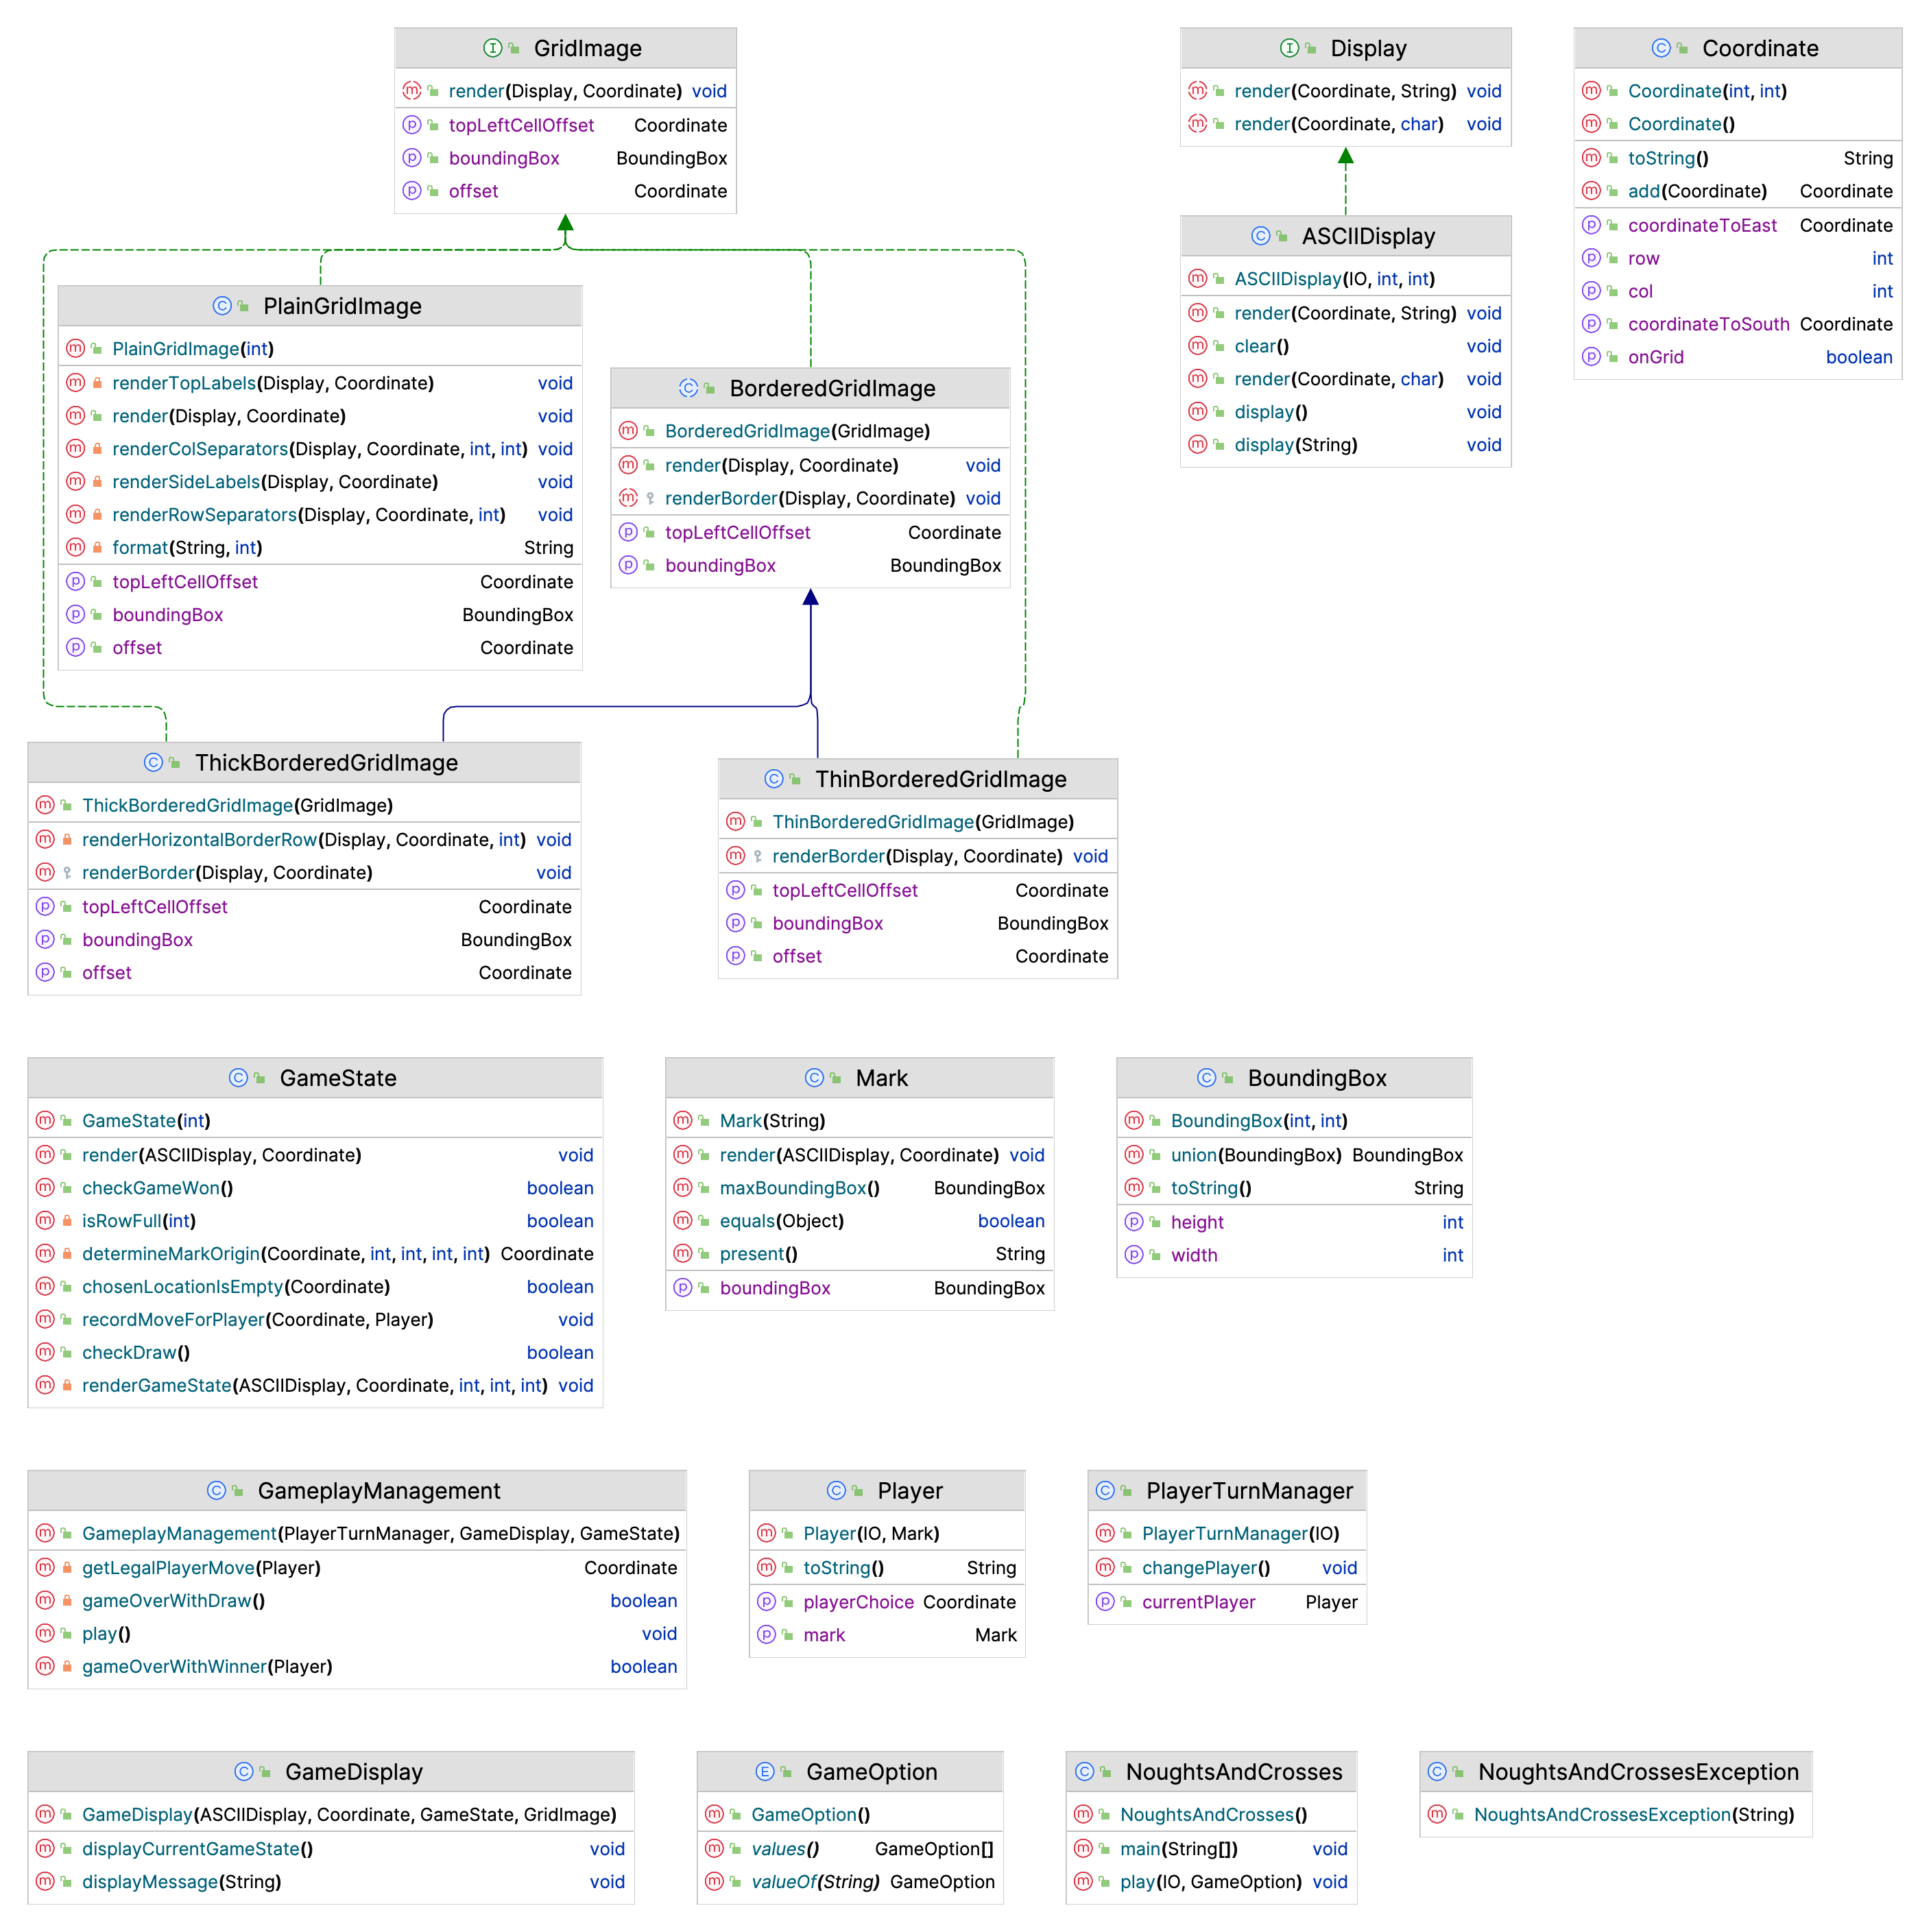
\includegraphics[width=18cm]{res/testuml.png}
    \caption{Test2 UML}
\end{figure}

在UML类图中单向关联用一个带箭头的直线表示。

双向关联就是双方各自持有对方类型的成员变量。在UML类图中,双向关联用一个不带箭头的直线表示。

自关联在UML类图中用一个带有箭头且指向自身的直线表示。

UML中聚合关系用带空心菱形和箭头的直线表示。聚合关系强调是“整体”包含“部分”,但是“部分”可以脱离“整体”而单独存在。比如汽车包含了发动机,而发动机脱离了汽车也能单独存在。

组合关系与聚合关系见得最大不同在于:这里的“部分”脱离了“整体”便不复存在,显然嘴是头的一部分且不能脱离了头而单独存在。在UML类图中,组合关系用一个带实心菱形和箭头的直线表示。

Driver的drive方法只有传入了一个Car对象才能发挥作用,因此我们说Driver类依赖于Car类。在UML类图中,依赖关系用一条带有箭头的虚线表示。

继承关系对应的是extend关键字,在UML类图中用带空心三角形的直线表示。

在UML类图中用带空心三角形的虚线表示实现关系。

\subsection{使用的设计模式}

\subsubsection{GridImage系列}

装饰器模式(Decorator Pattern): 这种设计模式允许在运行时向对象添加新功能,而不改变其结构。这种类型的设计模式属于结构模式,因为这种模式充当现有类的包装器。在这个例子中,BorderedGridImage 是一个装饰类,它增加了一个边框到基本的 GridImage 对象。ThickBorderedGridImage 和 ThinBorderedGridImage 是具体的装饰对象,它们分别添加了厚边框和薄边框。

组合模式(Composite Pattern): 通常用于表示对象的部分-整体层次结构。当你想要让客户端忽略单个对象与组合对象之间的差异时,就可以使用组合模式。GridImage 似乎是一个组合组件,它可以包含其他 GridImage 的实例,如 BorderedGridImage, ThickBorderedGridImage, 和 ThinBorderedGridImage。这些子类都继承自 GridImage 并可能有其自己的实现,形成了一个部分-整体的层次结构,这是组合模式的典型特征。

策略模式(Strategy Pattern): 这种模式涉及到算法的一个族系,能够相互替换,并让算法的变化独立于使用算法的客户。在这段代码中,GridImage 接口及其实现可能被视为策略模式的一部分,因为你可以根据需要在不同的 GridImage 实现之间进行切换,例如,你可以在 PlainGridImage、ThickBorderedGridImage 或 ThinBorderedGridImage 之间选择一个用于渲染。

\subsubsection{Display系列}

策略模式(Strategy Pattern):
在GameDisplay类中,GridImage和GameState作为参数传递到构造函数中,这表明了一种策略模式的使用。这个模式涉及将一系列算法(在这种情况下是渲染策略)定义为单独的类,然后在另一个类中使用它们。这允许算法的选择和变化不会影响到使用算法的类。在这里,GridImage和GameState可以是实现了特定接口的任何对象,GameDisplay不关心其内部工作方式,只是调用它们的render方法。这使得渲染逻辑可以在不更改GameDisplay类的情况下进行更改或扩展。

依赖注入(Dependency Injection):
GameDisplay类的构造函数接受ASCIIDisplay, Coordinate, GameState, 和GridImage对象作为参数,这是依赖注入的一种形式。依赖注入是一种允许类之间的依赖关系在运行时通过一个调用者来实现的设计模式。这增加了代码的模块化程度,使得单元测试更加容易,因为你可以传入模拟的依赖项来测试GameDisplay类的行为。
组合(Composition):

GameDisplay通过包含ASCIIDisplay, Coordinate, GameState, 和GridImage实例作为其属性,展示了组合的使用。组合是一种设计原则,它建议使用对象组合来实现新功能,而不是通过继承来扩展一个类的功能。GameDisplay类并没有从它的依赖项中继承功能,而是将它们组合在一起来实现新的功能。

\subsection{SOLID原则}

\subsubsection{GridImage系列 版本1}

单一职责原则 (Single Responsibility Principle, SRP):
GridImage 接口和它的实现类 PlainGridImage, BorderedGridImage, ThickBorderedGridImage, 和 ThinBorderedGridImage 都似乎遵循单一职责原则。每个类和接口都专注于网格图像的一个方面,无论是定义接口、处理无边框的图像、或是处理不同类型的边框。

开放封闭原则 (Open/Closed Principle, OCP):
这些类似乎也遵循开放封闭原则。例如,BorderedGridImage 是一个抽象类,可以被扩展来创建有不同边框的网格图像(如 ThickBorderedGridImage 和 ThinBorderedGridImage),而不需要修改现有代码。

里氏替换原则 (Liskov Substitution Principle, LSP):
从所给代码来看,子类似乎能够替代它们的基类。例如,任何需要 GridImage 的地方都可以使用 PlainGridImage、ThickBorderedGridImage 或 ThinBorderedGridImage,因为它们都遵循相同的接口。

接口隔离原则 (Interface Segregation Principle, ISP):
该原则建议将接口划分为更小的部分,避免强迫客户端实现它们不使用的方法。在这里,GridImage 接口似乎很简洁,只包含与网格图像相关的方法。不过,如果有些方法只适用于某些特定的图像,那么可能需要更多的接口来更好地隔离功能。

依赖反转原则 (Dependency Inversion Principle, DIP):
这些类似乎遵循依赖反转原则。例如,BorderedGridImage 依赖于 GridImage 接口而非 PlainGridImage 具体类。这意味着高级模块(如边框处理)不依赖于低级模块(如具体的网格图像实现),而是依赖于抽象。

\subsubsection{GridImage系列 版本2}

单一职责原则 (Single Responsibility Principle):
PlainGridImage 类似乎负责太多的呈现逻辑,如顶部标签、侧边标签、列分隔符和行分隔符的渲染。这可能违反了单一职责原则,因为如果要更改标签或分隔符的显示方式,你需要修改这个类。将这些职责分解为单独的类或方法可能会更好。

开放封闭原则 (Open/Closed Principle):
使用 GridImage 接口和如 BorderedGridImage 的抽象类,以及它们的具体实现如 ThickBorderedGridImage 和 ThinBorderedGridImage,项目似乎遵循了开放封闭原则。这是因为你可以通过创建新的 GridImage 实现来扩展网格的显示,而无需修改现有代码。

里氏替换原则 (Liskov Substitution Principle):
这些类似乎都遵循了里氏替换原则,因为它们都是从同一个接口 (GridImage) 继承而来,并且似乎可以互换使用,而不会影响程序的行为。

接口隔离原则 (Interface Segregation Principle):
GridImage 接口可能没有完全遵循接口隔离原则。这个接口为实现它的类施加了多种职责(获取边界框、获取偏移量、渲染等)。如果某个类只需要接口的部分功能,则该原则可能被违反。然而,在这个特定情况下,这似乎是必要的,因为所有的功能都是紧密相关的。

依赖倒置原则 (Dependency Inversion Principle):
类似乎都是依赖于 GridImage 这一抽象,而不是具体的实现,这是遵循依赖倒置原则的。然而,PlainGridImage 类直接与 Display 类交互,这意味着它依赖于一个具体的类而不是一个接口。如果 Display 是一个接口,并且具体的显示技术是它的实现,那么这将更好地遵循依赖倒置原则。

\subsubsection{Display系列}

S(Single Responsibility Principle,单一职责原则):
Display接口负责定义渲染方法,这是一个单一的职责。但是,它提供了两种不同的render方法,一种接受char,另一种接受String。这可能表明该接口承担了多重职责,尽管这两种方法都是渲染,但它们操作的数据类型不同。
GameDisplay类负责管理游戏的显示,包括渲染网格图像和游戏状态。这个类似乎有两个责任:管理游戏的显示和传递消息。虽然这些都与显示有关,但管理游戏状态的显示和通用消息传递可能被视为不同的职责。

O(Open/Closed Principle,开闭原则):
Display接口是开放的,因为可以实现新的Display类而无需修改接口。
GameDisplay类似乎对修改关闭,因为要改变显示的行为,你需要修改类的代码。然而,它对扩展是开放的,因为你可以通过传递不同的GridImage或GameState来改变渲染的外观和行为。

L(Liskov Substitution Principle,里氏替换原则):
从提供的代码中看不出违反此原则的明显迹象。然而,实际上是否符合此原则取决于实现Display接口的具体类的行为,以及如何使用GameDisplay类。

I(Interface Segregation Principle,接口隔离原则):
Display接口可能没有完全遵循接口隔离原则,因为它为不同类型的渲染(字符和字符串)定义了方法。如果某些类只需要一种渲染方法,这可能会迫使实现不需要的方法。

D(Dependency Inversion Principle,依赖倒置原则):
GameDisplay依赖于Display、GridImage和GameState的抽象,而不是具体实现,这符合依赖倒置原则。

\subsection{代码功能解析}

\subsubsection{Display 和 GameDisplay}

Display 是一个接口,用于定义渲染字符和字符串到某个坐标的方法。这是一个通用的、抽象级别的界面,可以被实现来显示游戏的不同部分。其定义了两个方法:
void render(Coordinate coord, char ch);:此方法接受一个 Coordinate 对象(代表在屏幕上的某个位置)和一个字符,然后将该字符渲染到指定的坐标。
void render(Coordinate coord, String str);:此方法与上一个类似,但它接受一个字符串而不是单个字符。这可以用于渲染字符串到特定的坐标。
由于 Display 只是一个接口,所以它不提供这些方法的具体实现。该接口的实现将依赖于具体的类(如可以将字符和字符串渲染到控制台、图形用户界面(GUI)或其他类型的显示)。

GameDisplay 是一个类,用于处理游戏的显示。它不直接实现 Display 接口,而是使用一个 Display 类型的对象(在这种情况下是 ASCIIDisplay 类型,该类型假定是 Display 接口的一个实现)。GameDisplay 负责管理和渲染游戏状态以及与玩家交互的其他界面元素。其成员变量包括:
\_origin:一个 Coordinate 对象,指示游戏渲染的起始点。
\_display:一个 ASCIIDisplay 对象,用于实际的渲染工作。假定 ASCIIDisplay 实现了 Display 接口。
\_gridImage:一个 GridImage 对象,代表游戏的网格。这可能是一个复杂的图像,表示游戏的棋盘。
\_gameState:一个 GameState 对象,维护游戏的当前状态(如哪个玩家的回合,棋盘上的哪些位置已经被占据等)。
该类具有以下方法:
public void displayCurrentGameState():此方法清除当前显示,重新渲染网格和游戏状态,然后显示它们。它使用 \_display、\_gridImage 和 \_gameState 成员变量来完成这些任务。
public void displayMessage(String message):此方法简单地在 \_display 上显示一条消息,可能是关于游戏状态的信息,例如“玩家X获胜”或“轮到玩家O”。
总的来说,Display 接口定义了渲染的基本合同,而 GameDisplay 类则利用这一合同来管理和显示游戏的具体状态和信息。

\subsection{对UML类图的解析}





